\section{Analiza Wymagań}

Firma AnyCode planuje przeniesienie swojej siedziby do zaadaptowanego budynku mieszkalnego i rozpoczęcie działalności w branży IT. W związku z tym, konieczne jest dokładne określenie wymagań dotyczących infrastruktury teleinformatycznej. Poniżej przedstawiamy analizę tych wymagań.

\section{Lokalizacja}

    Budynek Dom w srebrzykach 2 (G) \\
    ul. Przykładowa 2\\
    75-900 Koszalin\\

    \begin{flushleft}
        Poniżej znajdują się schematy techniczne budynku: 

        \begin{figure}[!htb]
            \centering
            \begin{minipage}{0.8\textwidth}
                \centering
                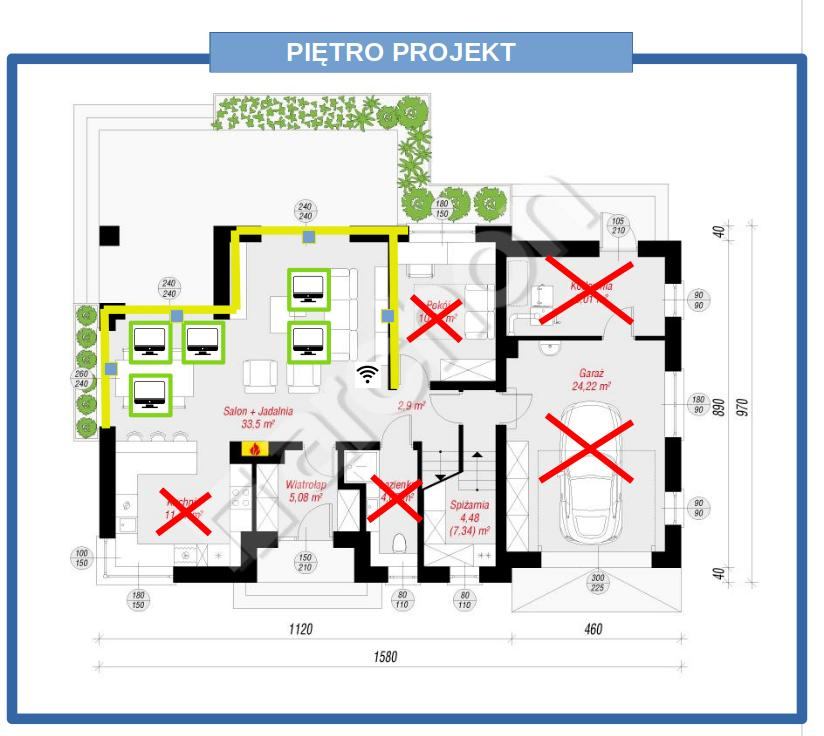
\includegraphics[width=\linewidth]{schematy/parter}
                \caption{Rzut: parteru}
            \end{minipage}
        \end{figure}

        \begin{figure}[!htb]
            \centering
            \begin{minipage}{0.8\textwidth}
                \centering
                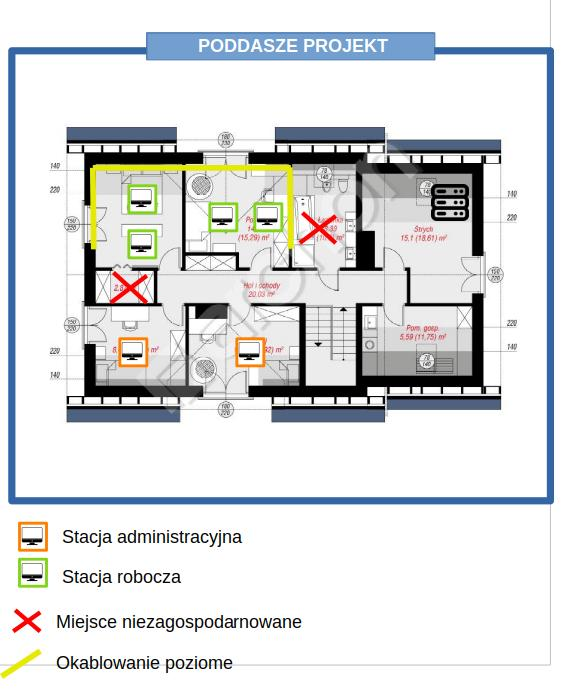
\includegraphics[width=\linewidth]{schematy/poddasze}
                \caption{Rzut poddasza}
            \end{minipage}
        \end{figure}

    \end{flushleft}


\subsection{Określenie Funkcji Pomieszczeń}

Budynek mieszkalny zostanie zaadaptowany na cele firmy AnyCode, obejmując różne rodzaje pomieszczeń. Wymagane funkcje pomieszczeń to:
- Biura dla zespołów programistycznych.
- Sale konferencyjne do spotkań z klientami i prezentacji projektów.
- Sala serwerowa do przechowywania i zarządzania danymi oraz aplikacjami.
- Przestrzeń kuchenna dla pracowników.
- Toalety i pomieszczenia socjalne.
- Inne pomieszczenia, takie jak recepcja i obszar relaksu.

\subsection{Technologie i Rozwiązania Sprzętowe}

Firma planuje skorzystać z nowoczesnych technologii i rozwiązań sprzętowych w swojej infrastrukturze teleinformatycznej. Obejmuje to:
- Wykorzystanie technologii Gigabit Ethernet (1GbE) do budowy sieci LAN.
- Użycie kabli UTP kat. 6 oraz światłowodu dla skomunikowania urządzeń.
- Wdrożenie zaawansowanych przełączników i routerów w celu zapewnienia wysokiej wydajności sieci.
- Implementację telefonii VoIP na każdym stanowisku komputerowym.
- Zakup i konfigurację centralnego serwera zasobów do przechowywania danych i aplikacji.
- Umowę z zewnętrzną firmą hostingową do utrzymania zasobów firmowych, w tym hosting serwisu www oraz poczty elektronicznej.

\subsection{Specyfikacja Urządzeń i Sprzętu}

W celu sprostania wymaganiom projektu, firma będzie musiała zakupić następujący sprzęt i urządzenia:
- Stacje robocze z odpowiednią wydajnością i konfiguracją dla programistów.
- Stacje administracyjne dla zarządzania siecią i serwerem.
- Drukarka sieciowa umożliwiająca drukowanie dokumentów z dowolnego stanowiska.
- Skaner do digitalizacji dokumentów.
- Urządzenia sieciowie

\subsection{Telefonia VoIP}

Telefonia VoIP zostanie wdrożona na każdym stanowisku komputerowym. W tym celu firma planuje zakup odpowiedniego oprogramowania oraz urządzeń telefonicznych dostosowanych do technologii VoIP.

\subsection{Centralny Serwer Zasobów}

Centralny serwer zasobów zostanie wykorzystany do przechowywania i zarządzania danymi firmowymi oraz aplikacjami. Będzie on zapewniał dostęp do zasobów dla wszystkich pracowników.

\subsection{Hosting Zewnętrzny}

Firma AnyCode podpisze umowę z zewnętrznym dostawcą usług hostingowych, OVH, który będzie utrzymywał zasoby firmowe, w tym hosting serwisu www oraz poczty elektronicznej.
\\

\includegraphics[width=0.3\textwidth]{ovh} \\
